%%%%%%%%%%%%%%%%%%%%%%%%%%%%%%%%%%%%%%%%%%%%%%%%%%%%%%%%%%%%%%%%%%%%%%%%%%%%%%%%%%%%%%%%%%%%%%%%%%%
%%%%%%%%%%%%%%%%%%%%%%%%%%%%%%%%%%%%%%%%%%%%%%%%%%%%%%%%%%%%%%%%%%%%%%%%%%%%%%%%%%%%%%%%%%%%%%%%%%%
%%%%%%%%%%%%%%%%%%%%%%%%%%%%%%%%%%%%%%%%%%%%%%%%%%%%%%%%%%%%%%%%%%%%%%%%%%%%%%%%%%%%%%%%%%%%%%%%%%%
%%%%%%%%%%%%%%%%%%%%%%%%%%%%%%%%%%%%%%%%%%%%%%%%%%%%%%%%%%%%%%%%%%%%%%%%%%%%%%%%%%%%%%%%%%%%%%%%%%%

\chapter{Metodología}

El presente trabajo resulta de una colaboración con el departamento de Gerontología, dependiente 
del Instituto de Ciencias de la Salud (ICSA).
Parte de esta colaboración incluye el acceso a los registros de PSG obtenidos por Vázquez Tagle 
y colaboradores en 2016 \cite{VazquezTagle16}; por ello, se cita la metodología de aquél estudio 
de la manera más fiel posible.
Así mismo se describe, a nivel de implementación, el análisis central de este trabajo: la prueba 
de Priesltey-Subba Rao. 

%%%%%%%%%%%%%%%%%%%%%%%%%%%%%%%%%%%%%%%%%%%%%%%%%%%%%%%%%%%%%%%%%%%%%%%%%%%%%%%%%%%%%%%%%%%%%%%%%%%
%%%%%%%%%%%%%%%%%%%%%%%%%%%%%%%%%%%%%%%%%%%%%%%%%%%%%%%%%%%%%%%%%%%%%%%%%%%%%%%%%%%%%%%%%%%%%%%%%%%

\section{Participantes y su diagnóstico}

Los sujetos fueron elegidos usando un muestreo no probabilístico de sujetos tipo \cite{Garcia09},
firmando un consentimiento informado previamente a su inclusión en el estudio. 
De manera extensiva, los criterios de exclusión para el estudio fueron los siguientes:
\begin{itemize}
\item Firma del consentimiento informado
\item Edad entre 60 y 85 años
\item Diestros (mano derecha dominante)
\item Sin ansiedad, depresión ni síndromes focales
\item No usar medicamentos o sustancias para dormir
\item Voluntario para el registro de PSG
\end{itemize}

Un total de 9 participantes cumplieron todos los criterios de exclusión y procedieron al registro 
de PSG; adicionalmente se tomó registro de otros tres adultos mayores, bajo el consentimiento de 
éstos y de los responsables del proyecto.

Usando los resultados obtenidos, los sujetos se dividieron en tres grupos:
\begin{description}
\item[Grupo PDC] (4 sujetos) Puntuación en Neuropsi menor a la media menos 3 desviaciones 
estándar, reportadas para poblaciones control \cite{Solis03}
\item[Grupo Control] (5 sujetos) Sin deterioro cognitivo
\item[Grupo Excluido] (3 sujetos) No satisfacen los criterios de inclusión, pero que se 
sometieron voluntariamente al estudio con aprobación de los responsables
\end{description}

Con respecto al tercer grupo, se conforma de sujeto que fallan en exactamente uno de los criterios 
de inclusión: FGH padece parálisis facial y posiblemente daño cerebral, MGG padece depresión, y EMT 
no califica como adulto mayor por su edad.
Se efectuaron los mismos análisis sobre este grupo con la finalidad de exhibir las capacidades y
limitaciones de las técnicas utilizadas, debido a lo cual este grupo es ignorado en la sección de 
resultados, pero retomado en la discusión.

\begin{table}
\centering
\bordes{1.1}
\begin{tabular}{c}
\textbf{Datos generales de los participantes}
\vspace{1em}
\end{tabular}
\begin{small}
\begin{tabular}{llcrrrrrrr}
\toprule
 \phantom{m}&
 & {Sexo} & {Edad} & {Esc.} & {Neuropsi} & {MMSE} & {SATS} & {KATZ} & {Gds} \\
\midrule
\multicolumn{6}{l}{{Grupo Control}}\\
&VCR    & F    & 59   & 12   & 107      & 29   & 21   & 0    & 3 \\
&MJH    & F    & 72   & 9    & 113      & 30   & 18   & 0    & 0 \\
&JAE    & F    & 78   & 5    & 102      & 28   & 19   & 0    & 5 \\
&GHA    & M    & 65   & 9    & 107.5    & 30   & 23   & 0    & 7 \\
&MFGR   & F    & 67   & 11   & 110      & 30   & 18   & 0    &   \\
\rowcolor{gris}
&\multicolumn{1}{c}{$\widehat{\mu}$} & 
              & 68.20& 9.20 & 107.90   & 29.40& 19.80& 0.00 & 3.00\\
\rowcolor{gris}
&\multicolumn{1}{c}{$\widehat{\sigma}$} & 
              & 7.19 & 2.68 & 4.07     & 0.89 & 2.17 & 0.00 & 3.08\\
\midrulec
%\hline
\multicolumn{6}{l}{{Grupo PDC}}\\
&CLO    & F    & 68   & 5    & 81       & 28   & 22   & 1    & 6 \\
&RLO    & F    & 63   & 9    & 90       & 29   & 20   & 0    & 3 \\
&RRU    & M    & 69   & 9    & 85       & 27   & 10   & 0    & 3 \\
&JGZ    & M    & 65   & 11   & 87       & 25   & 20   & 0    & 1 \\
\rowcolor{gris}
&\multicolumn{1}{c}{$\widehat{\mu}$} & 
              & 66.25& 8.50 & 85.75   & 27.25& 18.00& 0.25 & 3.25\\
\rowcolor{gris}
&\multicolumn{1}{c}{$\widehat{\sigma}$} & 
              & 2.75 & 2.52 & 3.77    & 1.71 & 5.42 & 0.50 & 2.06\\
\midrulec
%\hline
\multicolumn{6}{l}{{Sujetos excluidos}}\\
&FGH    & M    & 71   & 9    & 83.5     & 21   & 23   & 0    & 4  \\
&MGG    & F    & 61   & 9    & 114      & 28   & 29   & 1    & 14 \\
&EMT    & M    & 50   & 22   & 106      & 30   & 15   & 0    & 4  \\
\bottomrule
\end{tabular} 
\end{small}
\label{tab_sujetos}
\caption{Resultados de las pruebas neuropsicológicas 
}
\end{table}

%%%%%%%%%%%%%%%%%%%%%%%%%%%%%%%%%%%%%%%%%%%%%%%%%%%%%%%%%%%%%%%%%%%%%%%%%%%%%%%%%%%%%%%%%%%%%%%%%%%
%%%%%%%%%%%%%%%%%%%%%%%%%%%%%%%%%%%%%%%%%%%%%%%%%%%%%%%%%%%%%%%%%%%%%%%%%%%%%%%%%%%%%%%%%%%%%%%%%%%

\section{Registro del polisomnograma}

Los adultos mayores participantes fueron invitados a acudir a las instalaciones de la Clínica 
Gerontológica de Sueño (ubicadas dentro del Instituto de Ciencias de la Salud) para llevar a cabo 
el registro. Los participantes recibieron instrucciones de realizar una rutina normal de 
actividades durante la semana que precedió al estudio, y se les recomendó que no ingirieran 
bebidas alcohólicas o energizantes (como café o refresco) durante las 24 horas previas al 
experimento, ni durmieran siesta ese día.

El protocolo de PSG incluye 19 electrodos de EEG, 4 electrodos de EOG para registrar movimientos 
oculares horizontales y verticales, y 2 electrodos de EMG colocados en los músculos 
submentonianos para registrar la actividad muscular. 
La colocación de los electrodos para registrar la actividad EEG se realizó siguiendo las 
coordenadas del Sistema Internacional 10-20.

Debido a problemas técnicos con el electroencefalógrafo, el registro se llevó a cabo a 512 Hz 
para algunos sujetos y a 200 Hz para otros; la recomendación de la AASM, de un mínimo de 128 
Hz, se satisface. 
Las señales fueron amplificadas (amplificador de alta ganancia en cadena), filtradas (filtro paso 
de banda de 0.5--30 Hz) y digitalizadas para su posterior análisis.
En la tabla \ref{frecuencias} se reportan la duración de estos registros para cada sujeto.

%Debido a un cambio en el polisomnógrafo 
%usado, la frecuencia de muestreo (en Hz) cambia entre sujetos.

\begin{table}
\centering
\bordes{1.2}
\begin{tabular}{c}
\textbf{Datos generales sobre los registros de PSG}
\vspace{1em}
\end{tabular}
\begin{tabular}{llcrrcrrr}
\toprule
    \phantom{m}&
    &\multirow{2}{*}{\bordes{1}\begin{tabular}{l}Frecuencia\\ muestreo\end{tabular}}
    \bordes{1.2}
    & \multicolumn{2}{c}{Total} & \phantom{l}   & \multicolumn{3}{c}{MOR*}\\
    \cmidrule{4-5}  \cmidrule{7-9}
    &&          &Puntos  &  Tiempo   &&Puntos  &  Tiempo   &  \% MOR \\
\midrule
\multicolumn{6}{l}{{Grupo Control}}\\
&VCR &200       & 5166000&   7:10:30 &&438000  &   0:36:30 & 8\% \\
&MJH &512       &15851520&   8:36:00 &&1950720 &   1:03:30 &12\% \\
&JAE &512       &13931520&   7:33:30 &&2626560 &   1:25:30 &19\% \\
&GHA &200       &6558000 &   9:06:00 &&330000  &   0:27:30 & 5\% \\
&MFGR&200       &4932000 &   6:51:00 &&570000  &   0:47:30 &12\% \\

\midrule

\rowcolor{gris}
\multicolumn{6}{l}{{Grupo PDC}}\\
\rowcolor{gris}
&CLO &512       &14499840&   7:52:00 &&2027520 &   1:06:00 &14\% \\
\rowcolor{gris}
&RLO &512       &12994560&   7:03:00 &&1520640 &   0:49:30 &12\% \\
\rowcolor{gris}
&RRU &200       &2484000 &   3:27:00 &&228000  &   0:19:00 & 9\% \\
\rowcolor{gris}
&JGZ &512       &18539520&  10:03:30 &&506880  &   0:16:30 & 3\% \\

\midrulec

\multicolumn{6}{l}{{Sujetos excluidos}}\\
&FGH &512       &6220800 &   3:22:30 &&337920  &   0:11:00 & 5\% \\
&MGG &512       &15820800&   8:35:00 &&2549760 &   1:23:00 &16\% \\
&EMT &512       &21857280&  11:51:30 &&721920  &   0:23:30 & 3\% \\
\bottomrule
\end{tabular}
\caption{Cantidad de datos registrados para cada sujeto. Dado que el sueño MOR aparece fragmentado,
se reporta la suma de tales tiempos.}
\label{frecuencias}
\end{table}

La clasificación de las diferentes fases del sueño en el registro PSG se realizó manualmente sobre 
épocas de EEG de 30 segundos siguiendo los criterios estandarizados de la AAMS \cite{Hori01}, 
mismas que fueron descritas anteriormente.

%%%%%%%%%%%%%%%%%%%%%%%%%%%%%%%%%%%%%%%%%%%%%%%%%%%%%%%%%%%%%%%%%%%%%%%%%%%%%%%%%%%%%%%%%%%%%%%%%%%
%%%%%%%%%%%%%%%%%%%%%%%%%%%%%%%%%%%%%%%%%%%%%%%%%%%%%%%%%%%%%%%%%%%%%%%%%%%%%%%%%%%%%%%%%%%%%%%%%%%

\section{Aplicación de la prueba PSR}

Los registros digitalizados de PSG fueron convertidos a formato de texto bajo la codificación 
ASCII, a razón de un archivo por cada canal. 
Las épocas MOR fueron señaladas en archivos a parte, uno por cada sujeto.

Como se mencionó en secciones anteriores, la prueba PSR está pensada para series de tiempo con 
media 0, varianza finita y espectro puramente continuo. Se espera que la segunda condición se 
cumpla para los registros de PSG; las otras dos condiciones fueron 'forzadas', sustrayendo la media 
y la componente periódica (estimadas) del proceso.
Para lo anterior, se usó el algoritmo no-paramétrico STL (Seasonal-Trend decomposition using 
Loess) \cite{Cleveland1990} y que está implementado en R bajo la función \texttt{stl()}.

La prueba PSR se encuentra implementado en R bajo la función \texttt{stationarity()} del paquete 
\texttt{fractal}.
Los resultados de la prueba PSR, aplicado a todas las épocas contenidas en los registros de PSG,
fueron almacenados para su análisis posterior.

En cada canal que conforma el PSG (EEG, EOG y EMG), cada época registrada fue clasificada como 
\textit{posiblemente estacionaria} (PE) si, usando la prueba PSR, no pudo rechazarse la hipótesis de 
estacionariedad ($\alpha < 0.05$), o como 'no-estacionaria' en caso contrario.
La cantidad de épocas PE en cada individuo, durante el sueño MOR y NMOR, se muestra en las 
tablas \ref{total_gpos_mor}, \ref{total_gpos_nmor} y \ref{total_gpos_total}. Debido a la gran 
variabilidad entre los sujetos para la duración del sueño MOR, no se consideró el total de 
épocas PE, sino la proporción de éstas en cada etapa de sueño; tales cantidades se muestran 
en las tablas \ref{gpos_mor}, \ref{gpos_nmor} y \ref{gpos_total}. 
Adicionalmente se han calculado promedios y desviaciones estándar para ambos grupos (Control y 
PDC).

\begin{figure}
\centering
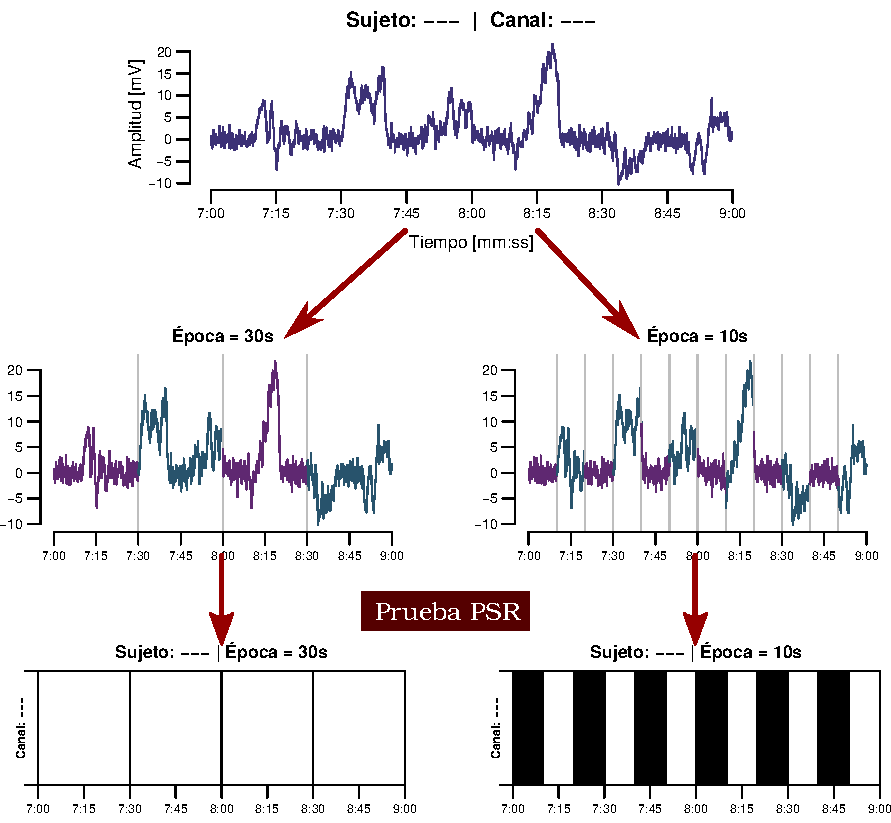
\includegraphics[width=\linewidth]{./img_diagramas/epocas_diferentes_v2.pdf}
\caption{Esquema de cómo se tomaron diferentes tamaños de época para estudiar los registros de 
PSG}
\label{epocas_diferentes}
\end{figure}



%%%%%%%%%%%%%%%%%%%%%%%%%%%%%%%%%%%%%%%%%%%%%%%%%%%%%%%%%%%%%%%%%%%%%%%%%%%%%%%%%%%%%%%%%%%%%%%%%%%
%%%%%%%%%%%%%%%%%%%%%%%%%%%%%%%%%%%%%%%%%%%%%%%%%%%%%%%%%%%%%%%%%%%%%%%%%%%%%%%%%%%%%%%%%%%%%%%%%%%
%%%%%%%%%%%%%%%%%%%%%%%%%%%%%%%%%%%%%%%%%%%%%%%%%%%%%%%%%%%%%%%%%%%%%%%%%%%%%%%%%%%%%%%%%%%%%%%%%%%
%%%%%%%%%%%%%%%%%%%%%%%%%%%%%%%%%%%%%%%%%%%%%%%%%%%%%%%%%%%%%%%%%%%%%%%%%%%%%%%%%%%%%%%%%%%%%%%%%%%